\documentclass[]{scrreprt}
\usepackage{amsmath,amsfonts,graphicx}
%\usepackage{multirow}
%\usepackage{pslatex}
%\usepackage{tabularx}
%\usepackage{comment}
%\usepackage{xspace}
%\usepackage{array}

%\usepackage{hyperref}

%\usepackage{caption}
%\DeclareCaptionFont{white}{\color{white}}
%\DeclareCaptionFormat{listing}{\colorbox{gray}{\parbox{\textwidth}{#1#2#3}}}

\def\species{\mathrm{sp}}
\def\phase{\mathrm{ph}}
\def\massfrac{\chi}
\def\flux{\mathbf{F}}
\def\darcyvel{\mathbf{v}}
\def\energydens{\mathcal{E}}
\def\d{\mathrm{d}}

\newcommand{\uo}{\mbox{UO\textsubscript{2}}\xspace}

\setcounter{secnumdepth}{3}


\begin{document}


\title{DiracKernel Tests}
\author{CSIRO}
\maketitle

\tableofcontents

\chapter{Geometric tests}

The test suite contains tests that demonstrate:
\begin{itemize}
\item when a point sink is placed at a node, it withdraws fluid (or heat) from only that node;
\item when a point sink that is proportional to mobility (or relative
  permeability, etc) is placed in an element where some nodes have
  zero mobility (or relative permeability, etc), then fluid (or heat)
  is not extracted from those nodes.
\end{itemize}

\chapter{Peaceman borehole fluxes}

The automatic test suite contains four tests that check that the Peaceman flux
\begin{equation}
f(P_{i}, x_{i}) =
W \left|C(P_{i}-P_{\mathrm{bh}})\right|
\frac{k_{\mathrm{r}}\rho}{\mu}(P_{i} - P_{\mathrm{bh}})
\label{bh.propto.eqn}
\end{equation}
is correctly implemented.  A vertical borehole is placed through the
centre of a single element, and fluid flow to the borehole as a
function of porepressure is measured.  The tests are
\begin{itemize}
\item A production borehole with $P_{\mathrm{bh}} = 0$, with a
  fully-saturated medium.
\item An injection borehole with $P_{\mathrm{bh}} = 10$\,MPa, with a
  fully-saturated medium.
\item A production borehole with $P_{\mathrm{bh}} = -1$\,MPa, with an
  unsaturated medium.
\item An injection borehole with $P_{\mathrm{bh}} = 0$, with an
  unsaturated medium.
\end{itemize}
The parameters common to these tests are:
\begin{center}
\begin{tabular}{|ll|}
\hline
Element size & $2\times 2\times 2$\,m$^{3}$ \\
Borehole radius & 0.1\,m \\
Permeability & $10^{-12}$\,m$^{2}$ \\
Gravity & 0 \\
Unit fluid weight & 0 \\
Fluid reference density & 1000\,kg.m$^{-3}$ \\
Fluid bulk modulus & 2\,GPa \\
Fluid viscosity & $10^{-3}$\,Pa.s \\
Van Genuchten $\alpha$ & $10^{-5}$\,Pa \\
Van Genuchten $m$ & 0.8  \\
Residual saturation & 0 \\
FLAC relperm $m$ & 2 \\
\hline
\end{tabular} \\
\end{center}
It is remotely possible that the MOOSE implementation {\em applies}
the borehole flux incorrectly, but {\em records} it as a Postprocessor
correctly as specified by Eqn~(\ref{bh.propto.eqn}).  Therefore, these
four simulations also record the fluid mass and mass-balance error in
order to check that the fluid mass is indeed being correctly changed
by the borehole.  Figure~\ref{bh02_05.fig} demonstrates that
Eqn~(\ref{bh.propto.eqn}) is indeed correctly implemented in MOOSE.

\begin{figure}[htb]
\centering
\begin{tabular}{cc}
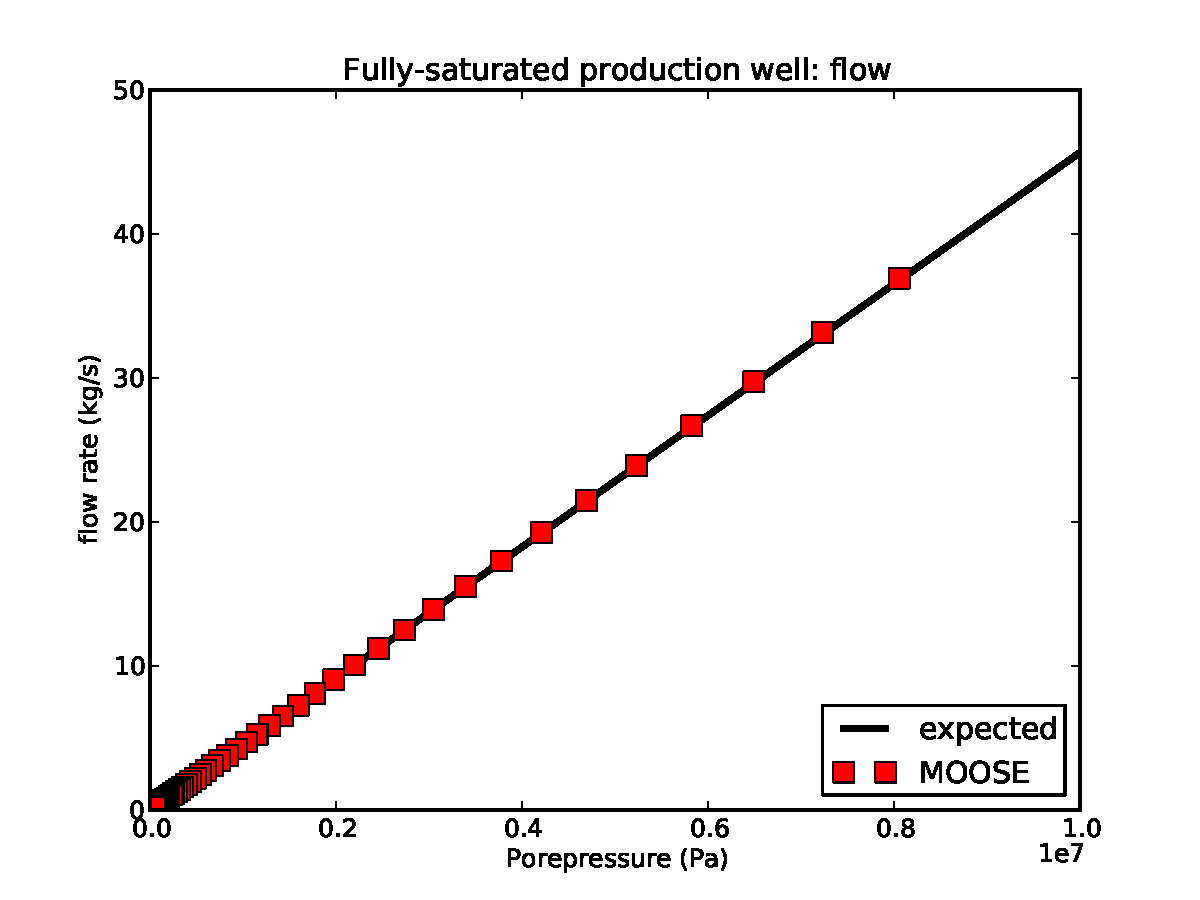
\includegraphics[width=7cm]{bh02_flow.pdf} &
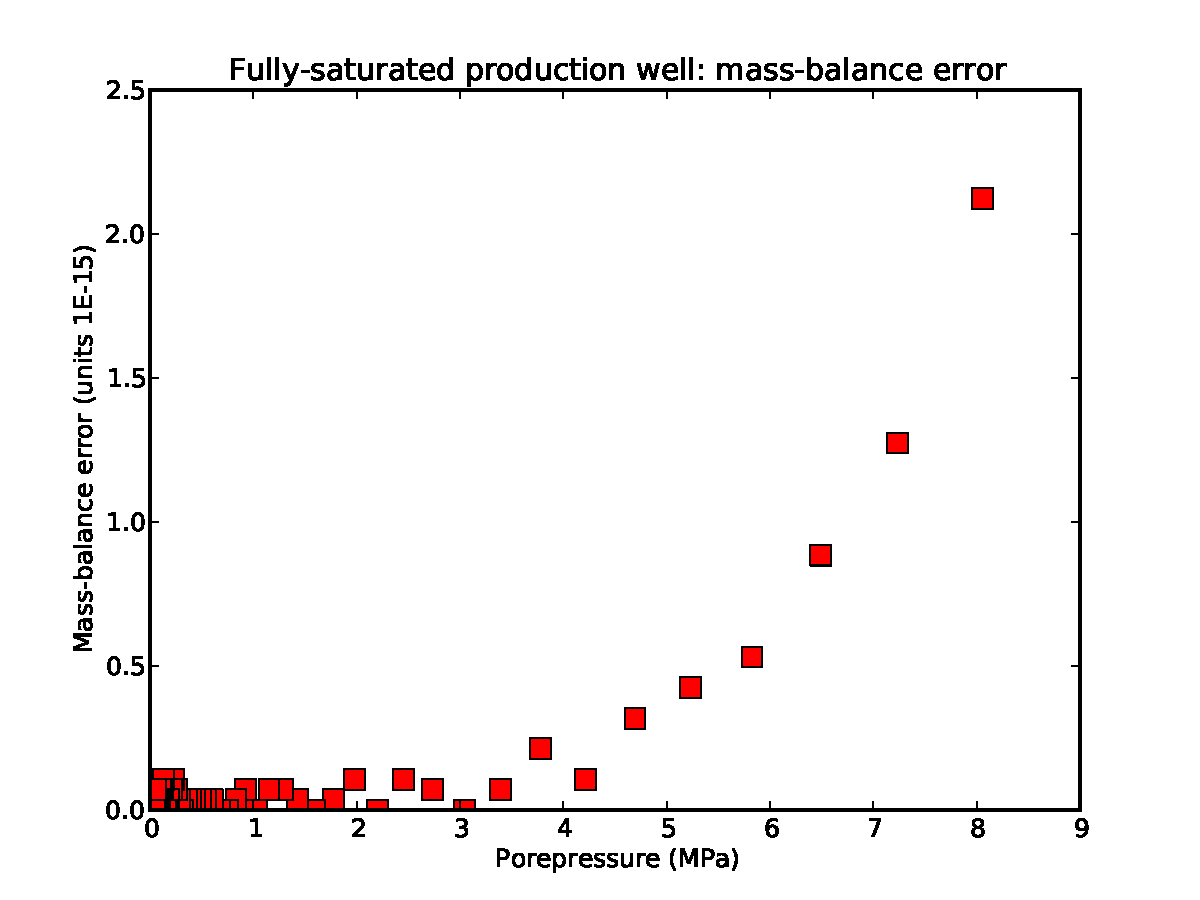
\includegraphics[width=7cm]{bh02_error.pdf} \\
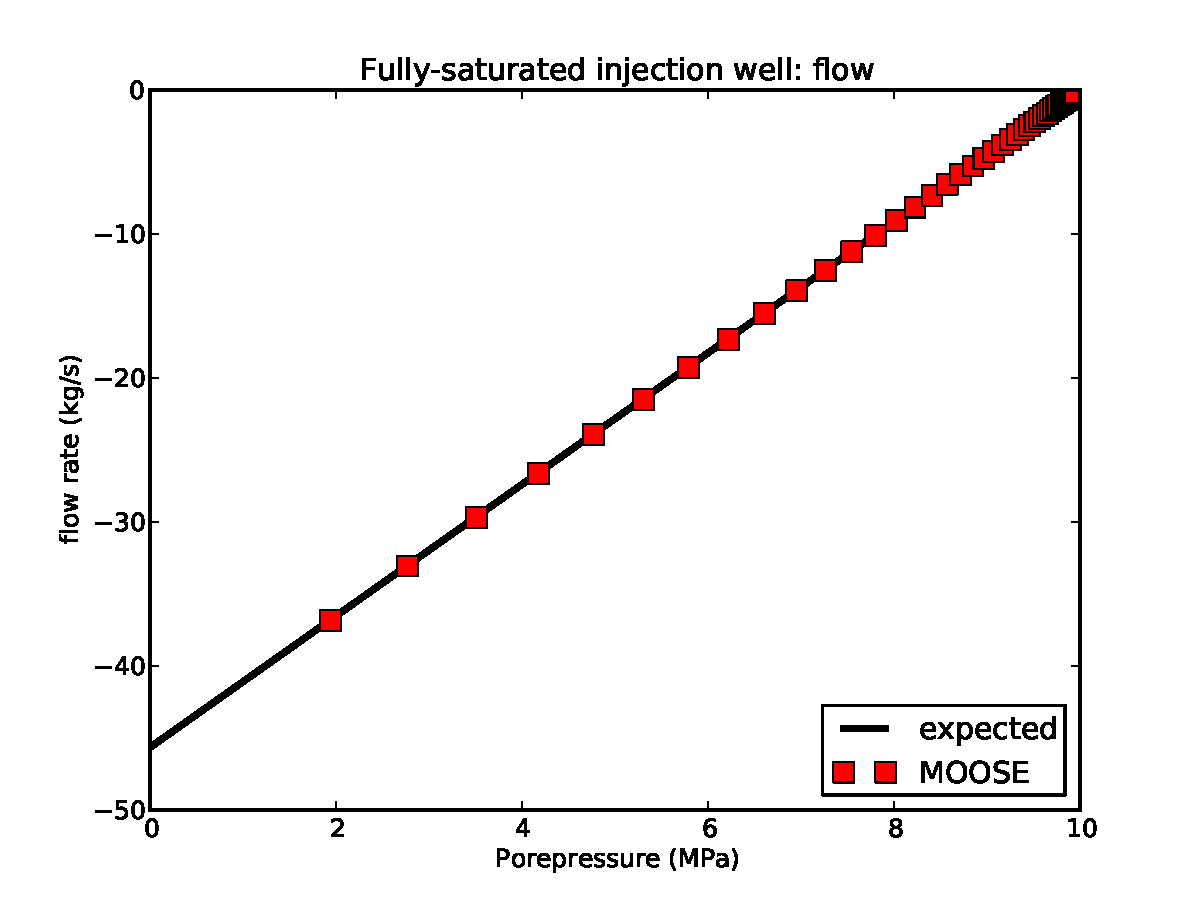
\includegraphics[width=7cm]{bh03_flow.pdf} &
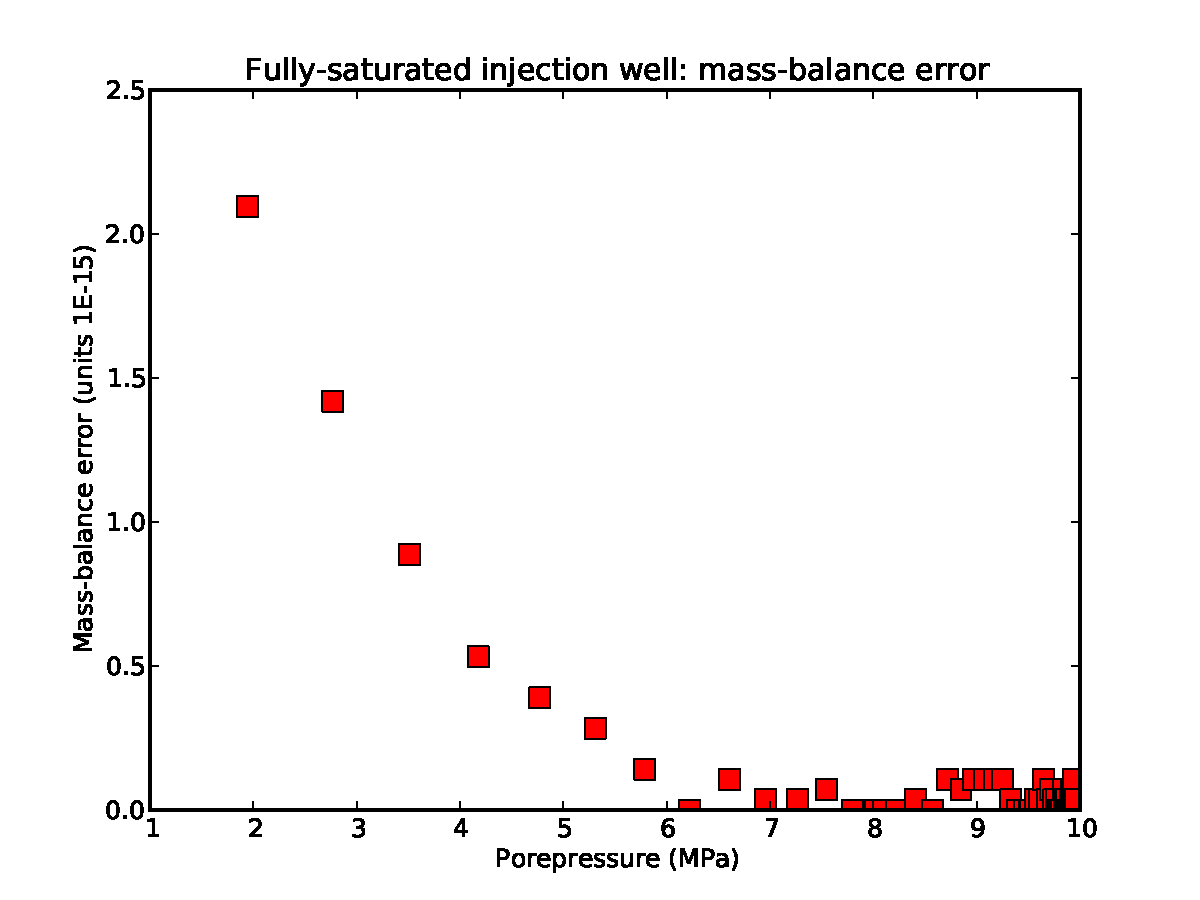
\includegraphics[width=7cm]{bh03_error.pdf} \\
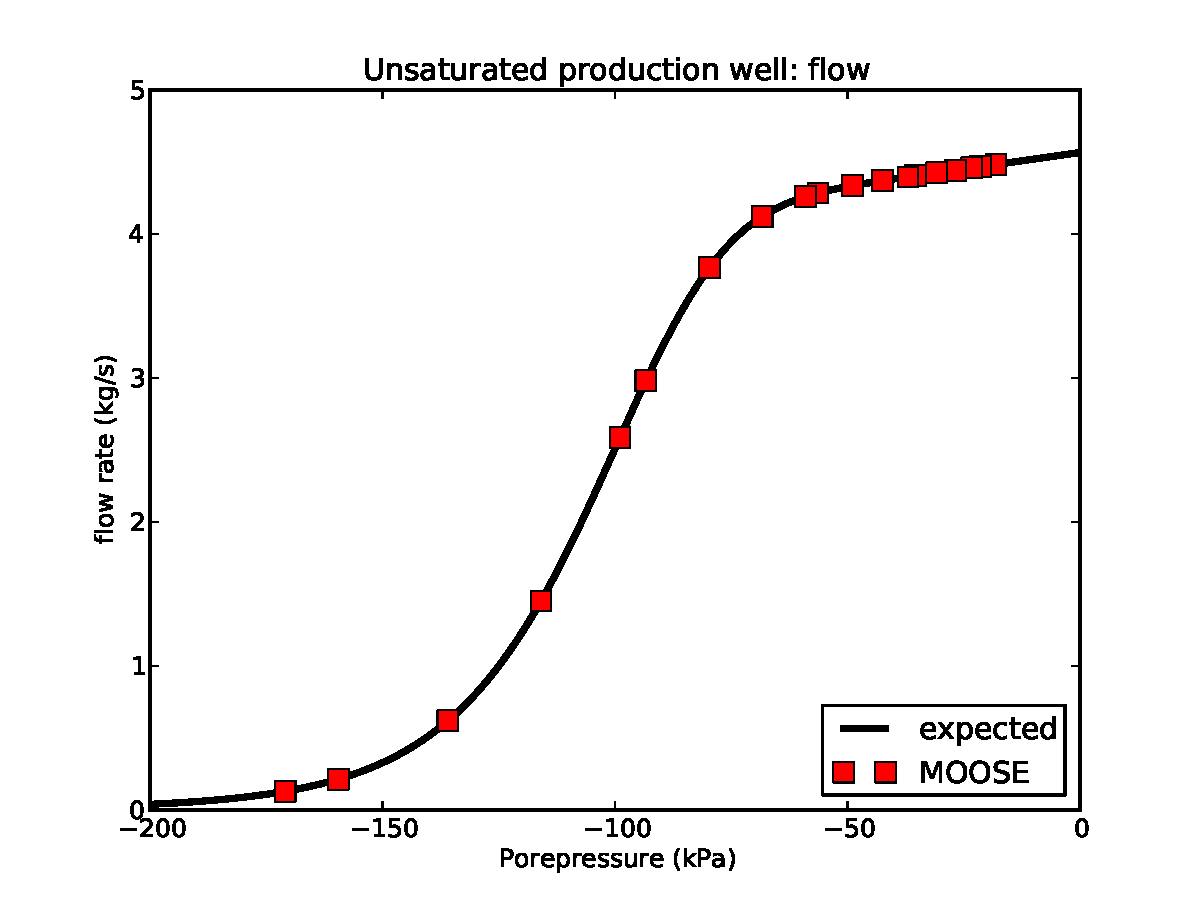
\includegraphics[width=7cm]{bh04_flow.pdf} &
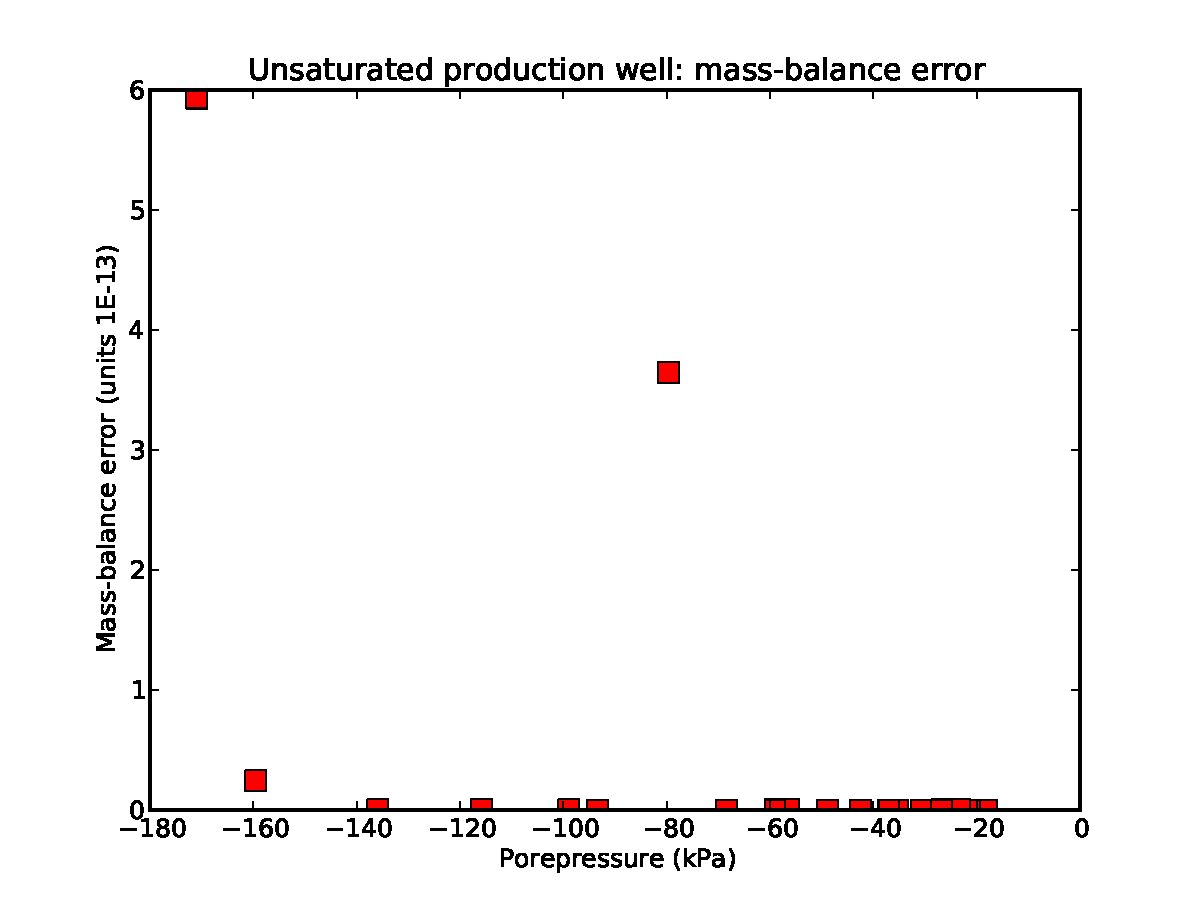
\includegraphics[width=7cm]{bh04_error.pdf} \\
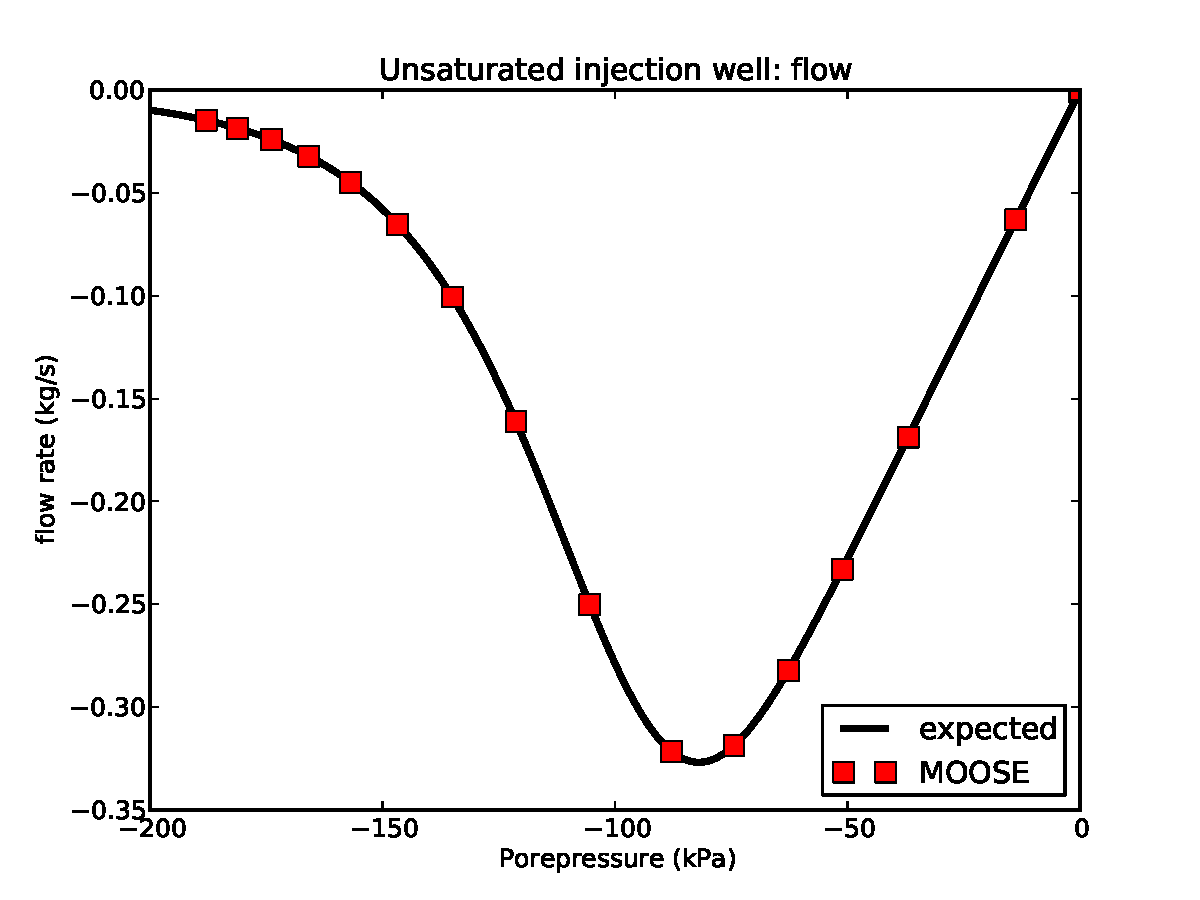
\includegraphics[width=7cm]{bh05_flow.pdf} &
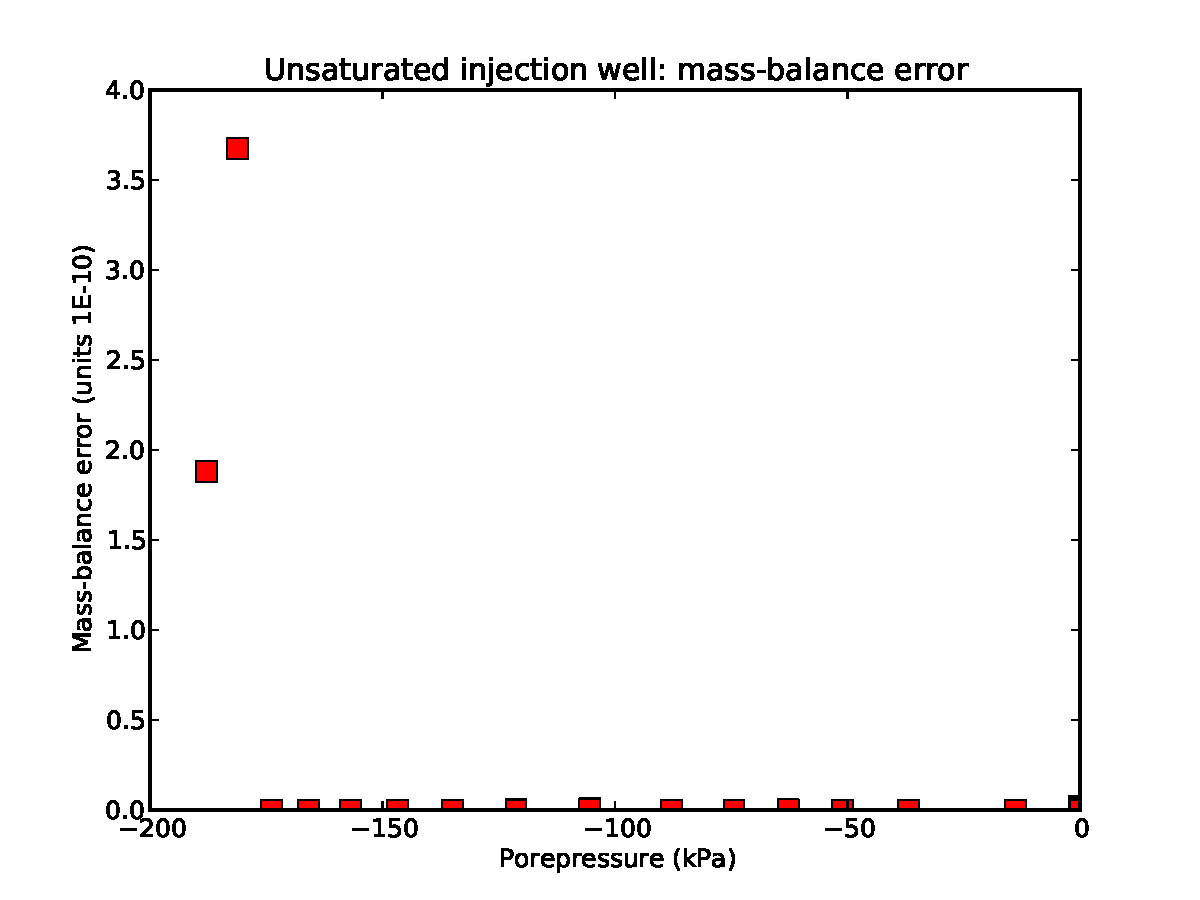
\includegraphics[width=7cm]{bh05_error.pdf} \\
\end{tabular}
\caption{Left figures: Comparison between the MOOSE result (in dots), and the
  expected behaviour of the borehole flux given by
  Eqn~(\ref{bh.propto.eqn}) (as a line) for the cases listed in the
  text.  Right
  figures: The mass balances, which are all small.}
\label{bh02_05.fig}
\end{figure}

\chapter{Comparison with analytic solution}
The Richards' equation for a fully-saturated medium with $\rho \propto
\exp(P/B)$ and large constant bulk modulus $B$ becomes Darcy's equation
\begin{equation}
\frac{\partial}{\partial t}\rho =  \nabla_{i}\alpha_{ij}\nabla_{j}\rho
\end{equation}
where $\alpha_{ij} = k_{ij}B/(\mu\phi)$, with notation described
in the Theory Manual.   In the isotropic case (where $k_{ij} =
\kappa \delta_{ij}$), the steadystate equation is just Laplace's
equation
\begin{equation}
\nabla^{2}\rho = 0 \ ,
\end{equation}
Place a borehole of radius $r_{\mathrm{bh}}$ and infinite length
oriented along the $z$ axis.  Then the situation becomes 2D and can be
solved in cylindrical coordinates, with $\rho=\rho(r,\theta)$ and
independent of $z$.  If the pressure at the borehole wall
$r=r_{\mathrm{bh}}$ is $P_{\mathrm{bh}}$, then the fluid density is
$\rho_{\mathrm{bh}} \propto \exp(P_{\mathrm{bh}}/B)$.  Assume that at
$r=R$ the fluid pressure is held fixed at $P_{R}$, or equivalently the
density is held fixed at $\rho_{R}$.  Then the solution of Laplace's
equation is well-known to be
\begin{equation}
\rho = \rho_{\mathrm{bh}} + (\rho_{R} - \rho_{\mathrm{bh}})
\frac{\log(r/r_{\mathrm{bh}})}{\log(R/r_{\mathrm{bh}})} \ .
\label{eqn.log.bh}
\end{equation}
This is the fundamental solution used by Peaceman and others to derive
expressions for $W$ by comparing with numerical expressions resulting
from Eqn~(\ref{bh.propto.eqn}) (see Theory Manual for more details).

Chen and Zhang (see Theory manual) have derived an expression for $W$
in the case where this borehole is placed at a node in a square mesh.
This test compares the MOOSE steadystate solution with a single
borehole with $W$ defined by 
Chen and Zhang's formula is compared with Eqn~(\ref{eqn.log.bh}) to
illustrate that the MOOSE implementation of a borehole is correct.

Figure~\ref{bh07.fig} shows this comparison.  Most parameters in this
study are identical to those given in the above table with the
following exceptions: the mesh is shown in Fig~\ref{bh07.mesh.fig};
the permeability is $10^{-11}$\,m$^{2}$; the borehole radius is 1\,m;
the borehole pressure is $P_{\mathrm{bh}}=0$; the outer radius is
$r=300$\,m; and the outer pressure is $P_{R}=10$\,MPa.

\begin{figure}[htb]
\centering
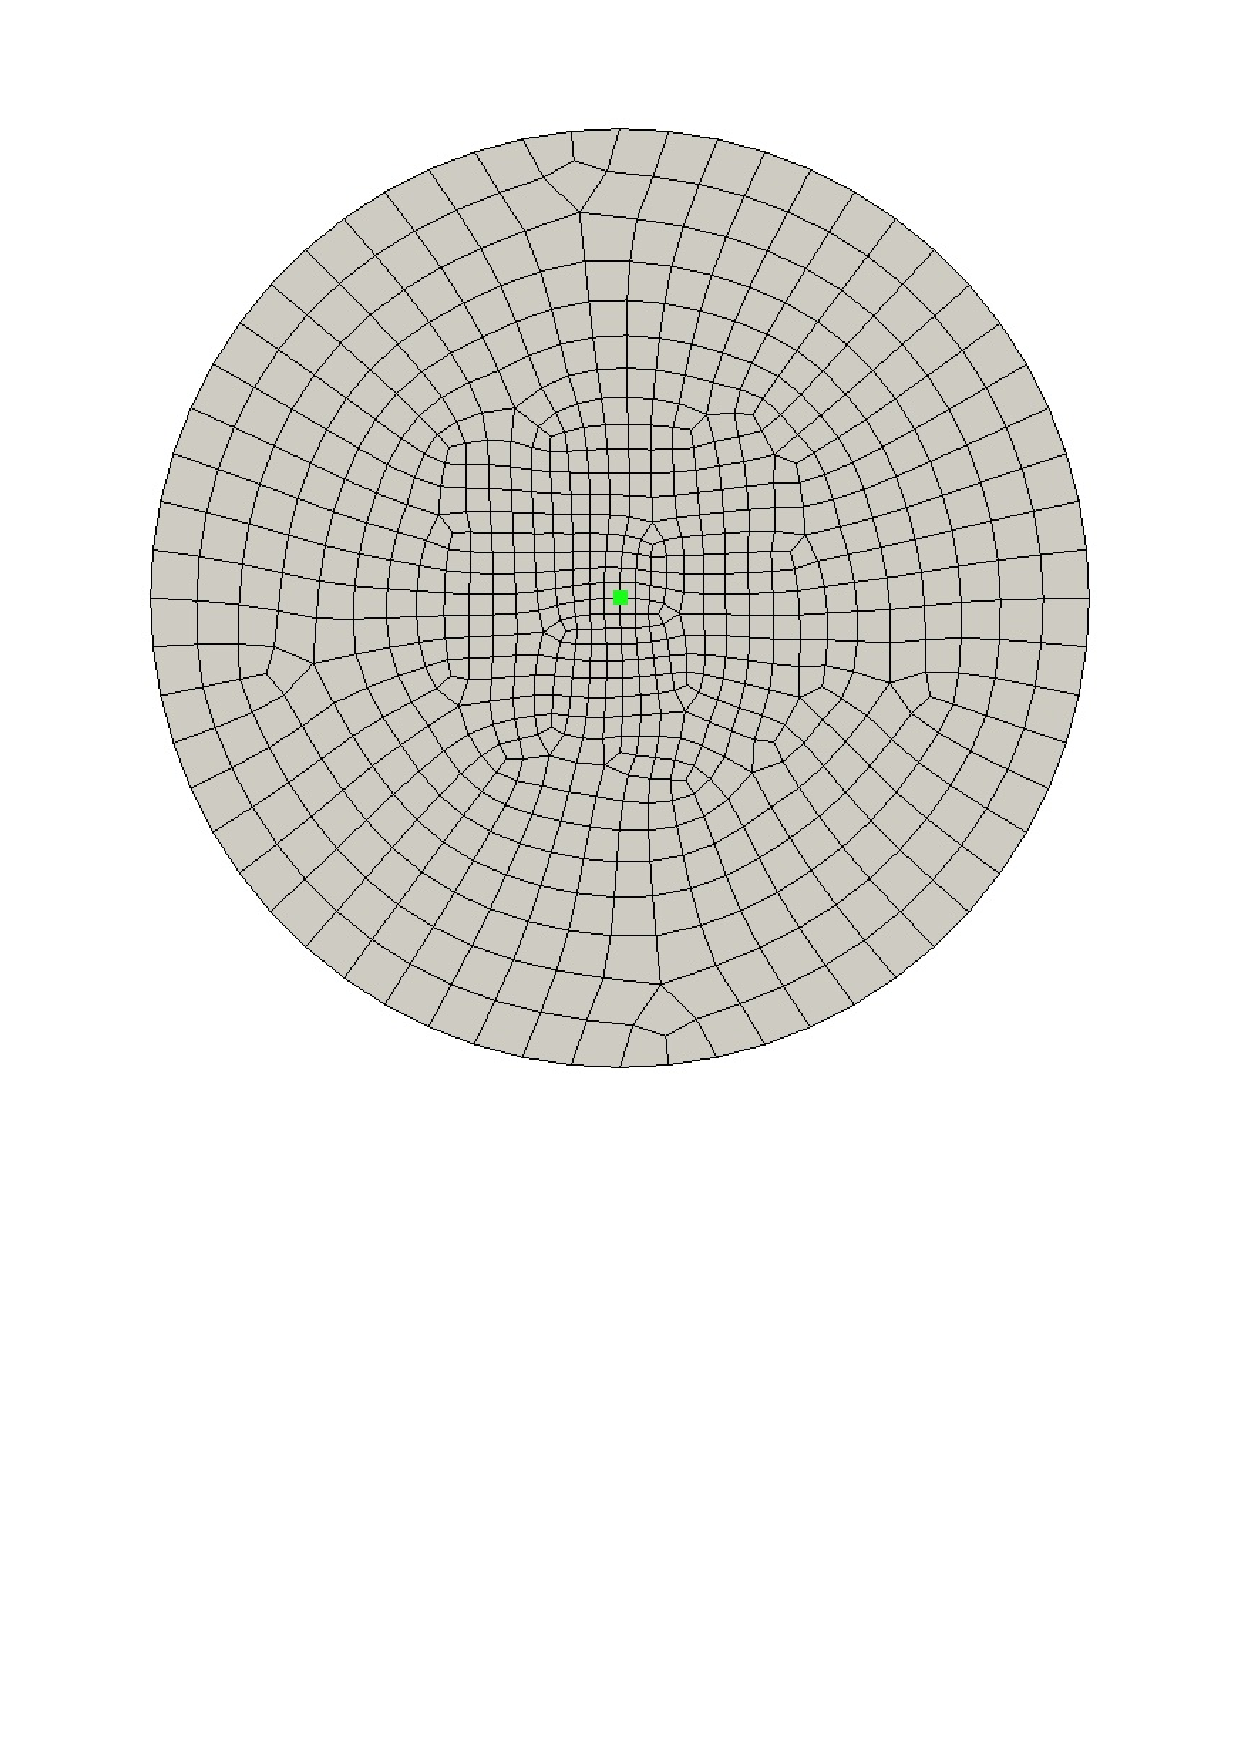
\includegraphics[width=8cm]{bh07_mesh.pdf}
\caption{The mesh used in the comparison with Eqn~(\ref{eqn.log.bh}),
  with the green dot indicating the position of the borehole.
  The central elements are $10\times 10$\,m$^{2}$, and the outer
  boundary is at $r=300$\,m.}
\label{bh07.mesh.fig}
\end{figure}



\begin{figure}[htb]
\centering
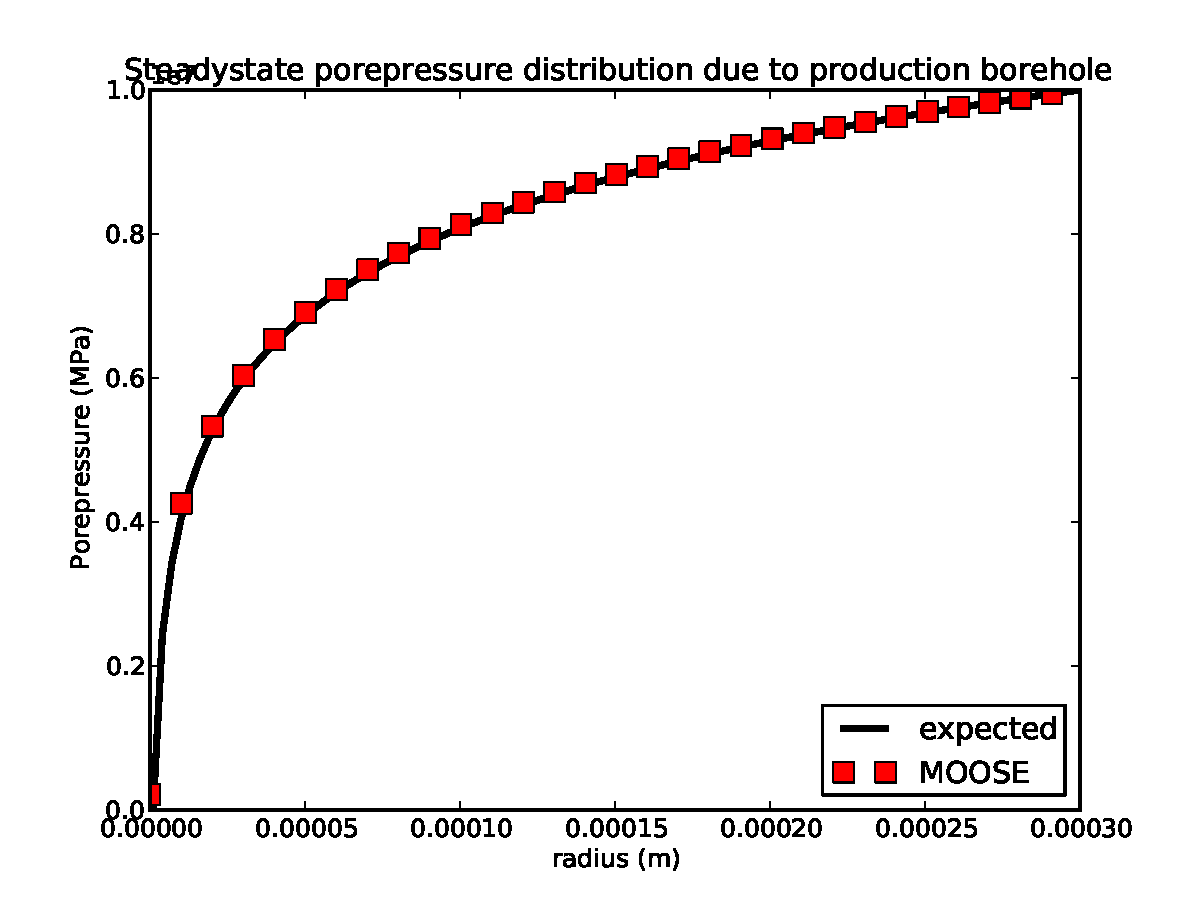
\includegraphics[width=12cm]{bh07.pdf}
\caption{Comparison of the MOOSE results (dots) with the analytical
  solution Eqn~(\ref{eqn.log.bh}) for the steadystate porepressure
  distribution surrounding single borehole.}
\label{bh07.fig}
\end{figure}



\end{document}

